\documentclass{beamer}
\mode<presentation>
\usepackage{amsmath}
\usepackage{amssymb}
\usepackage{bm}


%\usepackage{advdate}
\usepackage{adjustbox}
\usepackage{subcaption}
%\usepackage{enumitem}
\usepackage{enumerate}
\usepackage{multicol}
\usepackage{mathtools}
\usepackage{listings}
\usepackage{url}
\def\UrlBreaks{\do\/\do-}
\usetheme{Boadilla}
\usecolortheme{lily}
\setbeamertemplate{footline}
{
  \leavevmode%
  \hbox{%
  \begin{beamercolorbox}[wd=\paperwidth,ht=2.25ex,dp=1ex,right]{author in head/foot}%
    \insertframenumber{} / \inserttotalframenumber\hspace*{2ex} 
  \end{beamercolorbox}}%
  \vskip0pt%
}
\setbeamertemplate{navigation symbols}{}

\providecommand{\nCr}[2]{\,^{#1}C_{#2}} % nCr
\providecommand{\nPr}[2]{\,^{#1}P_{#2}} % nPr
\providecommand{\mbf}{\mathbf}
\providecommand{\pr}[1]{\ensuremath{\Pr\left(#1\right)}}
\providecommand{\qfunc}[1]{\ensuremath{Q\left(#1\right)}}
\providecommand{\sbrak}[1]{\ensuremath{{}\left[#1\right]}}
\providecommand{\lsbrak}[1]{\ensuremath{{}\left[#1\right.}}
\providecommand{\rsbrak}[1]{\ensuremath{{}\left.#1\right]}}
\providecommand{\brak}[1]{\ensuremath{\left(#1\right)}}
\providecommand{\lbrak}[1]{\ensuremath{\left(#1\right.}}
\providecommand{\rbrak}[1]{\ensuremath{\left.#1\right)}}
\providecommand{\cbrak}[1]{\ensuremath{\left\{#1\right\}}}
\providecommand{\lcbrak}[1]{\ensuremath{\left\{#1\right.}}
\providecommand{\rcbrak}[1]{\ensuremath{\left.#1\right\}}}
\providecommand{\rank}{\text{rank}}
\theoremstyle{remark}
\newtheorem{rem}{Remark}
\newcommand{\sgn}{\mathop{\mathrm{sgn}}}
\providecommand{\abs}[1]{\left\vert#1\right\vert}
\providecommand{\res}[1]{\Res\displaylimits_{#1}} 
\providecommand{\norm}[1]{\lVert#1\rVert}
\providecommand{\mtx}[1]{\mathbf{#1}}
\providecommand{\mean}[1]{E\left[ #1 \right]}
\providecommand{\fourier}{\overset{\mathcal{F}}{ \rightleftharpoons}}
%\providecommand{\hilbert}{\overset{\mathcal{H}}{ \rightleftharpoons}}
\providecommand{\system}{\overset{\mathcal{H}}{ \longleftrightarrow}}
	%\newcommand{\solution}[2]{\vec{Solution:}{#1}}
%\newcommand{\solution}{\noindent \vec{Solution: }}
\providecommand{\dec}[2]{\ensuremath{\overset{#1}{\underset{#2}{\gtrless}}}}
\newcommand{\myvec}[1]{\ensuremath{\begin{pmatrix}#1\end{pmatrix}}}
\newenvironment{amatrix}[1]{%
  \left(\begin{array}{@{}*{#1}{c}|c@{}}
}{%
  \end{array}\right)
}
\let\vec\mathbf

\lstset{
%language=C,
frame=single, 
breaklines=true,
columns=fullflexible
}

%\numberwithin{equation}{section}

\title{Matgeo-5.2.2}
\author{Harichandana Varanasi-ai25btech11039}

\date{\today} 
\begin{document}

\begin{frame}
\titlepage
\end{frame}

\section*{Outline}

\begin{frame}
\frametitle{Question}

\noindent\textbf{Q-5.2.2} \;
Solve the simultaneous linear equations
\[
5u-4v+8=0,\qquad 7u+6v-9=0 .
\]

\end{frame}
\begin{frame}{Solution}
   \renewcommand\theequation{\arabic{equation}}
\begin{align}
5u - 4v &= -8 \tag{1}\\
7u + 6v &= 9 \tag{2}
\end{align}

Writing in matrix form,
\begin{equation}
\myvec{5 & -4 \\ 7 & 6}\myvec{u \\ v}=\myvec{-8 \\ 9} \tag{3}
\end{equation}

Augmented matrix,
\begin{equation}
\myvec{5 & -4 & -8 \\ 7 & 6 & 9} \tag{4}
\end{equation}

\noindent Row operation: $R_2 \to 5R_2 - 7R_1$,
\begin{equation}
\myvec{5 & -4 & -8 \\ 0 & 58 & 101} \tag{5}
\end{equation}

\noindent Normalize second row: $R_2 \to \dfrac{R_2}{58}$,
\end{frame}
\begin{frame}{Solution}
\begin{equation}
\myvec{5 & -4 & -8 \\ 0 & 1 & \dfrac{101}{58}} \tag{6}
\end{equation}

\noindent Eliminate above: $R_1 \to R_1 + 4R_2$,
\begin{equation}
\myvec{5 & 0 & -\dfrac{30}{29} \\ 0 & 1 & \dfrac{101}{58}} \tag{7}
\end{equation}

\noindent Normalize first row: $R_1 \to \dfrac{R_1}{5}$,
\begin{equation}
\myvec{1 & 0 & -\dfrac{6}{29} \\ 0 & 1 & \dfrac{101}{58}} \tag{8}
\end{equation}
\end{frame}
\begin{frame}{Solution}

Thus, the solution vector is
\begin{equation}
\myvec{u \\ v}=\myvec{-\dfrac{6}{29} \\ \dfrac{101}{58}} \tag{9}
\end{equation}
\end{frame}


\begin{frame}{Plot}
  \begin{figure}[H]
  \centering
  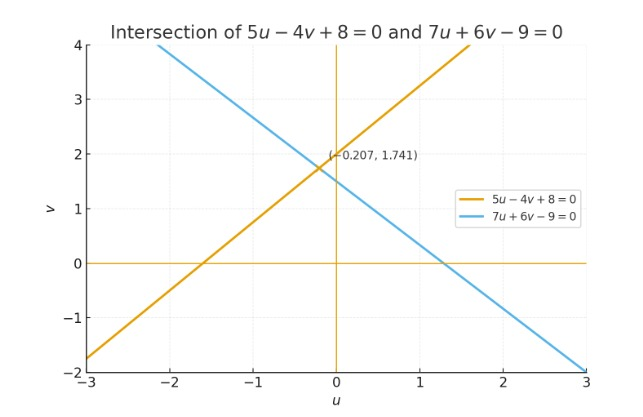
\includegraphics[width=0.8\linewidth]{figs/matgeo-5.2.2.jpeg}
  \caption{Intersection of $5u-4v+8=0$ and $7u+6v-9=0$ at
           $\left(-\tfrac{6}{29},\,\tfrac{101}{58}\right)$.}
  \label{fig:5.2.2}
\end{figure}
\end{frame}

\end{document}
